\setcounter{figure}{0}
\setcounter{table}{0}
\section{R峰检测算法及其实现}
\subsection{相关研究中的算法实现}
作为ECG信号处理中重要的一部分,R峰的检测算法虽然简单但也备受关注。相关研究往往将检测R峰作为信号处理的第一步,进行详细的阐述、实现和测试。

R峰指QRS波群中R波的出现,根据R峰峰值、采样速率及两次R峰出现的间隔时间等数据,可计算得出信号的心率、RR间期、心率波动情况等特征,同时R峰的检测也有助于对QRS波的定位。现有研究中涉及R峰检测的算法不胜枚举,其中大多数算法基于差分阈值法——即波形的斜率超过某一阈值则判定为出现R峰。同时为了减少各种干扰(肌电干扰、基线漂移等),这些算法均对信号进行了预处理。如\cite{_4.0android_2013}中采用四层连续小波变换和差分阈值法结合的方式确定R峰的出现;\cite{clifford_signal_2002}中使用带通滤波、时间平均、平方等预处理后,判断信号是否两次穿越基准点的方法;\cite{sadhukhan_r-peak_2012}中创新性地使用了一种经过滤波后求取两次差值的方法。虽然这些算法不尽相同,但容易归纳出它们的共同点:这些方法均针对R峰最显著的特征,即幅值突变。因此,这些方法本质上都属于对信号斜率的筛选。

以上算法均通过使用不同类型的ECG信号库验证了准确率,具有一定的稳定性和可靠性。但信号的突然抖动、基线漂移(主要体现在研究\cite{clifford_signal_2002}中)等异常可能影响这些算法的检测。因此本研究尝试实现一种更加稳定的R峰检测方法。

\subsection{基于局部最大值的R峰检测算法}

考虑到R峰的出现伴随着波形幅值的突变,通过检查ECG波形中的最大值,必然可以得到R峰。以此为基础设计R峰检测算法。首先使用长度为10的均值滤波器滤波,得到平滑的图形。该过程可表示为:

\begin{equation}
  {{e}_{avg}}[j-5]=\frac{\sum\limits_{j=6}^{n}{e[j-5]+e[j-4]+,\ldots ,+e[j+4]}}{10}
  \label{equ1}
\end{equation}

其中${{e}_{avg}}[n]$表示经过滤波的信号序列, 表示原始信号序列。此处理使得波形更加平滑,易于分析。之后检测信号中第一次R峰的出现:跳过信号序列前0.4s的数据后,选取长度为80的菲重叠窗口并取此窗口中信号的最大幅值,将其与上次窗口中的最大值比较,将较大值存入最大值缓存中,并将较大值对应窗口的数据平均值存入平均值缓存中,即:

\begin{equation}
\begin{aligned}
 & {{t}_{\max }}=\max ({{e}_{\max }}[i],{{e}_{\max }}[i-1]); \\ 
 & {{t}_{avg}}={\sum\limits_{i=0}^{79}{{{e}_{avg}}[j+i]}}/{80}\;  
\end{aligned}
\label{equ2}
\end{equation}

其中${{t}_{\max}}$表示最大值缓存,${{e}_{\max }}[i]$表示滑动窗口取得的最大值序列,${{t}_{avg}}$表示平均值缓存。判断每次窗口中的数据是否满足:

\begin{equation}
\frac{{{t}_{\max }}}{{{t}_{avg}}}>1.2
\label{equ3}
\end{equation}

若上述条件满足,则判定第一次R峰出现,记录下该次峰值,平移窗口进行后续判断。若不满足,则平移窗口,继续检验,直到出现满足条件的R峰。检测到第一次R峰出现后,剩余的步骤主要判断新出现的最大值是否与第一次R峰类似:

\begin{equation}
\left| \frac{{{t}_{\max }}-{{t}_{avg}}}{{{l}_{\max }}-{{l}_{avg}}}-1 \right|<0.5
\label{equ4}
\end{equation}

其中${{l}_{\max }}$和${{l}_{avg}}$分别代表最近一次窗口中取得的最大值与平均值。当上述条件满足时, ${{t}_{\max }}$中的值替换为${{l}_{\max }}$的值,${{l}_{\max }}$所在的点记录为一次R峰出现。继续这一步骤,直到整段信号分析完毕。至此,所有的R峰峰值及其出现时间均被记录,通过以下算法计算RR间期及心率:

\begin{equation}
\begin{aligned}
  & RR={{R}_{tl}}-{{R}_{te}}\times {{f}_{trans}}; \\ 
 & B=\frac{RR}{60}; \\ 
\end{aligned}
\label{equ5}
\end{equation}

其中$RR$代表$RR$间期,${{R}_{tl}}$代表后一次R峰出现时间,${{R}_{te}}$代表前一次R峰出现时间,${{f}_{trans}}$代表数据的传输速率,$B$代表心率。
	
分析\ref{equ3}和\ref{equ4}可看出,由于该算法比较了同一窗口中最大值与平均值的差值,而平均值随窗口的移动而波动,因此基线漂移所造成的R峰异常增高并不会影响到算法的判断——评判标准是基于“相对的”最大值,而不是“绝对的”。同时,由于第一次出现的R峰被采用为随后检测R峰的基准,那么之后的一些异常情况造成的突变也可以被避开。

\begin{figure}[htb]
  \centering
  \subfigure[数据源]{
    \label{fig4-1a} %% label for first subfigure
    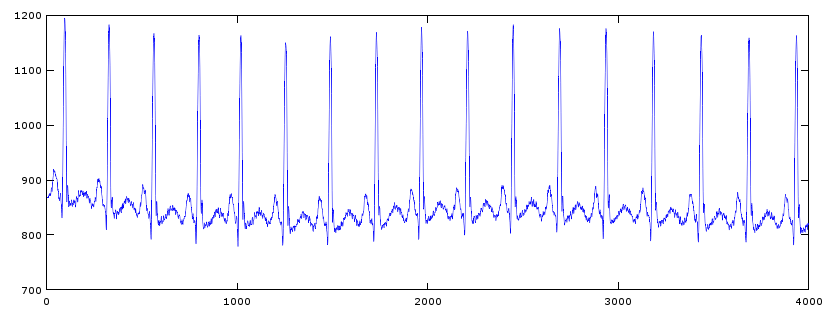
\includegraphics[width=0.8\textwidth]{fig4-1a.png}}
  \\
  \subfigure[经过平均滤波的波形]{
    \label{fig4-1b} %% label for second subfigure
    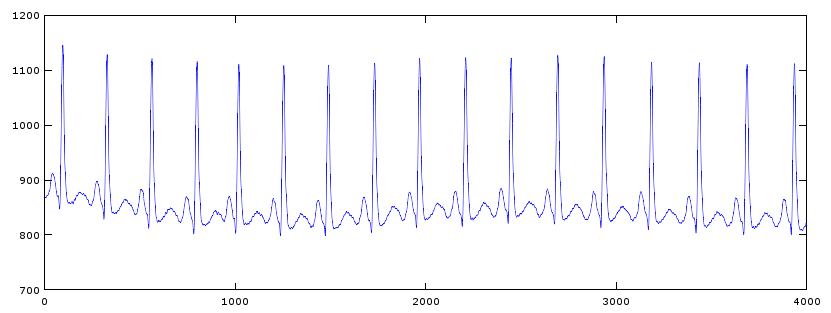
\includegraphics[width=0.8\textwidth]{fig4-1b.png}}
  \\
  \subfigure[算法识别出的R峰]{
    \label{fig4-1c} %% label for second subfigure
    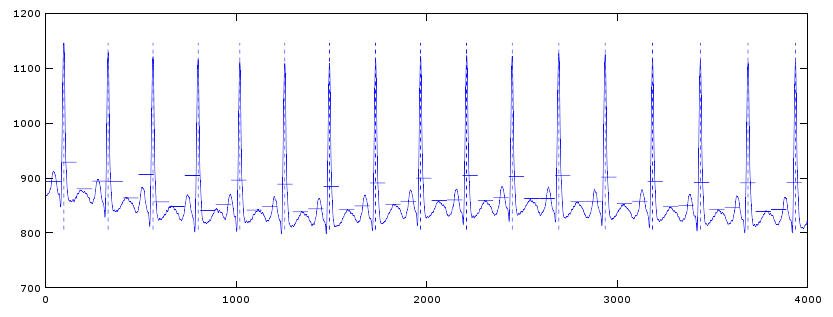
\includegraphics[width=0.8\textwidth]{fig4-1c.png}}
    \caption{ECG波形图的处理过程}
  \label{fig4-1} %% label for entire figure
\end{figure}

图\ref{fig4-1}分别展示了经过预处理和R峰探测后的ECG波形。可以看出,经过了平均滤波的波形明显更加平滑,同时基线漂移并没有影响到R峰的判定,因为每个窗口的平均值是随基线波动的。

本算法并未涉及小波变换等数据分析方法,在嵌入式设备等计算资源不那么丰富的平台上也能轻松运行;同时,算法的迭代次数并不高。因此该算法具有较理想的时间和空间复杂度,容易在Android平台实现。

\subsection{R峰检测算法的Java实现}
如前所述,在EcgDataAnalyzer类中实现成员类BeatRateAndRpeakDetectionThread线程和长度为80的数据分析缓存,当缓存空间满时启动线程,分析数据。在同一个窗口的处理中,单次for循环即可实现平均数和最大值的求取,其代码片段如下:

\begin{center}
\begin{lstlisting}
for (cnt = 0; cnt < 80; cnt++) {
    dataAvgValue += dataTemp[cnt].getData();
    if (rpeakLocalMax.getData() < dataTemp[cnt].getData()) {
        rpeakLocalMax = dataTemp[cnt];
    }
}
dataAvgValue = dataAvgValue / 80;
\end{lstlisting}
\end{center}

其中数据的获取方法getData()经synchronized关键字修饰,可防止两次R峰检测对最大值缓存的并发访问,也因此防止了某几次耗时稍长的检测影响下一次检测。至此,信号的预处理完成。接下来线程进行R峰的检测。

\begin{center}
\begin{lstlisting}
double RRinterval = (recentRpeak.getDataId() -lastRpeak.getDataId()) * EcgData.RECORDRATE;
beatRate = 60 / RRinterval;
lastRpeak = recentRpeak;
Message uiRefreshMessage = Message.obtain();
uiRefreshMessage.what = 3;
uiRefreshMessage.arg1 = (int) beatRate;
uiRefreshMessage.arg2 = (int) (RRinterval*100);
uiRefreshHandler.sendMessage(uiRefreshMessage);
\end{lstlisting}
\end{center}
当线程检测到R峰出现时调用rpeaksHandling(DataTemp)方法处理数据。DataTemp数据类包含了R峰峰值及其出现的时间,使用前一节所述方法计算出RR间期与心率后,使用Handler机制传递给主线程数据,主线程负责稍后的显示。相关代码如上所示。

\subsection{本章小结}
本章从介绍现有R峰检测算法开始,简述了现行大多数R峰检测算法,并对这些算法进行了归纳。在第二节,简述了所提出算法的原理,并且展示了算法在实际应用中的效果。最后简要介绍了算法的Java实现过程中进行优化的部分,也介绍了RR间期与心率计算的Java实现代码。

本章算法测试部分将在第五章介绍。
